% Intended LaTeX compiler: pdflatex
\documentclass[10pt,a4paper,UTF8]{article}
\usepackage{zclorg}
\usepackage{tikztheorem}
\author{zcl.space}
\date{}
\title{用两种方法证明 \(\sqrt{2}\) 是无理数}
\hypersetup{
 pdfauthor={zcl.space},
 pdftitle={用两种方法证明 \(\sqrt{2}\) 是无理数},
 pdfkeywords={PMA},
 pdfsubject={用两种方法证明 \(\sqrt{2}\)是无理数},
 pdfcreator={Emacs 25.0.50.1 (Org mode 9.1.2)},
 pdflang={English}}
\begin{document}

\maketitle
\tableofcontents
\titlepic{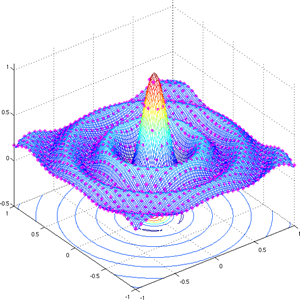
\includegraphics[scale=0.25]{../../img/sinc.PNG}}

\section{引言}
\label{sec:orgba4bfa4}


牛顿和莱布尼茨为微积分这一强大工具的发明权展开了旷日持久的争论,然而当他们争论的时候,人们还没有为微积分奠定分析学基础。虽然工程师已经使用微积分解决了诸多问题,直到Dedekind等人建立了严密的实数统,数学家才“放心”的接受微积分。建立实数统的过程是从整数向有理数再向无理数扩展的过程。从有理数向无理数扩充的过程中, 一个著名的问题是:证明\(\sqrt{2}\)是一个无理数。 \(\sqrt{2}\)是一个无理数告诉人们在任意两个有理数之间除了有无数个有理数外还有一些不是有理数的数,这些数就是像\(\sqrt{2}\)一样的无理数。

本文用两种方法证明\(\sqrt{2}\)是一个无理数。这两种方法都基于反证法,第一种反证法比较常见,我大概高中的时候知道了,第二种反证法基于集合论。
\section{第一种证明方法}
\label{sec:org582964e}


假设存在一个有理数 \(p\) ,满足
\begin{equation}
\label{eq:pequal2}
p^{2} = 2
\end{equation}

有理数 \(p\) 可以被写作 \(p=m/n\),其中 \(m\) 和 \(n\) 是整数,而且我们可以选择 \(m\) 和 \(n\)使得这两个数没有除1以外的公约数。这样式(\ref{eq:pequal2})变为:
\begin{equation}
\label{eq:2}
m^{2} = 2n^{2}
\end{equation}

从式(\ref{eq:2})可以看出, \(m^{2}\) 是一个偶数,所以 \(m\) 是一个偶数,所以 \(m^{2}\)能被4整除。进而说明 \(n^{2}\)也是偶数, \(n\)也是偶数。 \(m\)和 \(n\)都是偶数与\(m\)和 \(n\)的最大公因数是1矛盾。进而推出 \(p=m/n\)不是有理数。
\section{第二种证明方法}
\label{sec:orgf9ea3a6}


第一种证明方法在高中学习反证法的时候就有所涉及,第二种方法却不是很常见,不过也是基于反证法。

令 \(A\) 是使 \(p^{2}<2\) 的一切正有理数 \(p\)的集合。令 \(B\) 是使 \(p^{2}>2\) 的一切正有理数 \(p\)的集合。我们来证明 \(A\)中没有最大数, \(B\)中没有最小数。更确切的说对于 \(A\)中的每个 \(p\),能在 \(A\)中找到一个有理数 \(q\),使得\(p {<} q\),并且对于 \(B\) 中的每个 \(p\) 都有一个 \(q\) ,使得 \(p {>} q\) .

现在,为每一个有理数 \(p\) 配置一个数 \(q\),使得
\begin{equation}
\label{eq:q}
q = p - \frac{p^{2}-2}{p+2}= \frac{2p+2}{p+2}
\end{equation}
所以有:
\begin{equation}
\label{eq:q2}
q^{2} -2 = \frac{2(p^{2}-2)}{(p+2)^{2}}
\end{equation}
如果 \(p\) 在 \(A\) 中,则\(p^{2}<2\),而式(\ref{eq:q})说明 \(q {>} p\), 式(\ref{eq:q2})说明\(q^{2}<2\).因此\(q\) 在 \(A\) 中。这说明对于\(A\) 中的任何一个数 \(p\)总能找到一个数 \(q\)使得 \(q {>} p\),也即 \(A\)中没有最大值.

如果 \(p\) 在 \(B\) 中,则\(p^{2}>2\),而式(\ref{eq:q})说明 \(q {<} p\), 式(\ref{eq:q2})说明\(q^{2}>2\).因此\(q\) 在 \(B\) 中。这说明对于\(B\) 中的任何一个数 \(p\)总能找到一个数 \(q\)使得 \(q {<} p\),也即 \(A\)中没有最小值.
\section{尾声}
\label{sec:org63881f3}


以上的讨论说明尽管两个有理数之间还会存在无数个有理数,但是两个有理数之间除了无数个有理数之外还有某些空隙,无理数并没有占满实数轴。这些数是无理数,无理数和有理数共同构成了实数系,这也是实数系在分析学中起基础作用的原因。

第二种方法从集合论出发完成证明。在学习集合论,数学分析的过程中,我们还会用到类似的思路。
\end{document}
